\documentclass[border=8pt]{standalone}
\usepackage{fontspec}
\setmainfont{TeX Gyre Heros}
\setsansfont{TeX Gyre Heros}
\usepackage{tikz}
\usetikzlibrary{arrows.meta,positioning,shapes.geometric,shapes.misc,shapes.symbols,fit,backgrounds,calc,chains}
\definecolor{ink}{HTML}{111827}
\definecolor{band}{HTML}{F3F4F6}
\definecolor{band2}{HTML}{E5E7EB}
\definecolor{accent}{HTML}{1D4ED8}
\definecolor{accentlight}{HTML}{DBEAFE}
\definecolor{warn}{HTML}{B91C1C}
\definecolor{warnlight}{HTML}{FEE2E2}
\definecolor{ok}{HTML}{047857}
\definecolor{oklight}{HTML}{D1FAE5}
\tikzset{
  >={Stealth[length=2.6mm]},
  box/.style={draw=ink, line width=0.6pt, rounded corners=9pt, fill=white, align=center,
              inner sep=4pt, font=\small},
  pill/.style={box, rounded corners=13pt},
  key/.style={box, fill=accentlight, draw=accent, line width=0.9pt},
  soft/.style={box, fill=band},
  dec/.style={draw=ink, line width=0.6pt, diamond, aspect=2.2, align=center, inner sep=1.5pt,
              font=\footnotesize, fill=white},
  arr/.style={->, draw=ink, line width=0.6pt},
  darr/.style={->, draw=ink, line width=0.6pt, dashed},
  lbl/.style={font=\footnotesize, fill=white, inner sep=1.5pt},
  layer/.style={draw=band2, fill=band, rounded corners=6pt},
  title/.style={font=\bfseries\small, align=left, anchor=west},
}
\begin{document}
\sffamily\hyphenpenalty=10000\exhyphenpenalty=10000

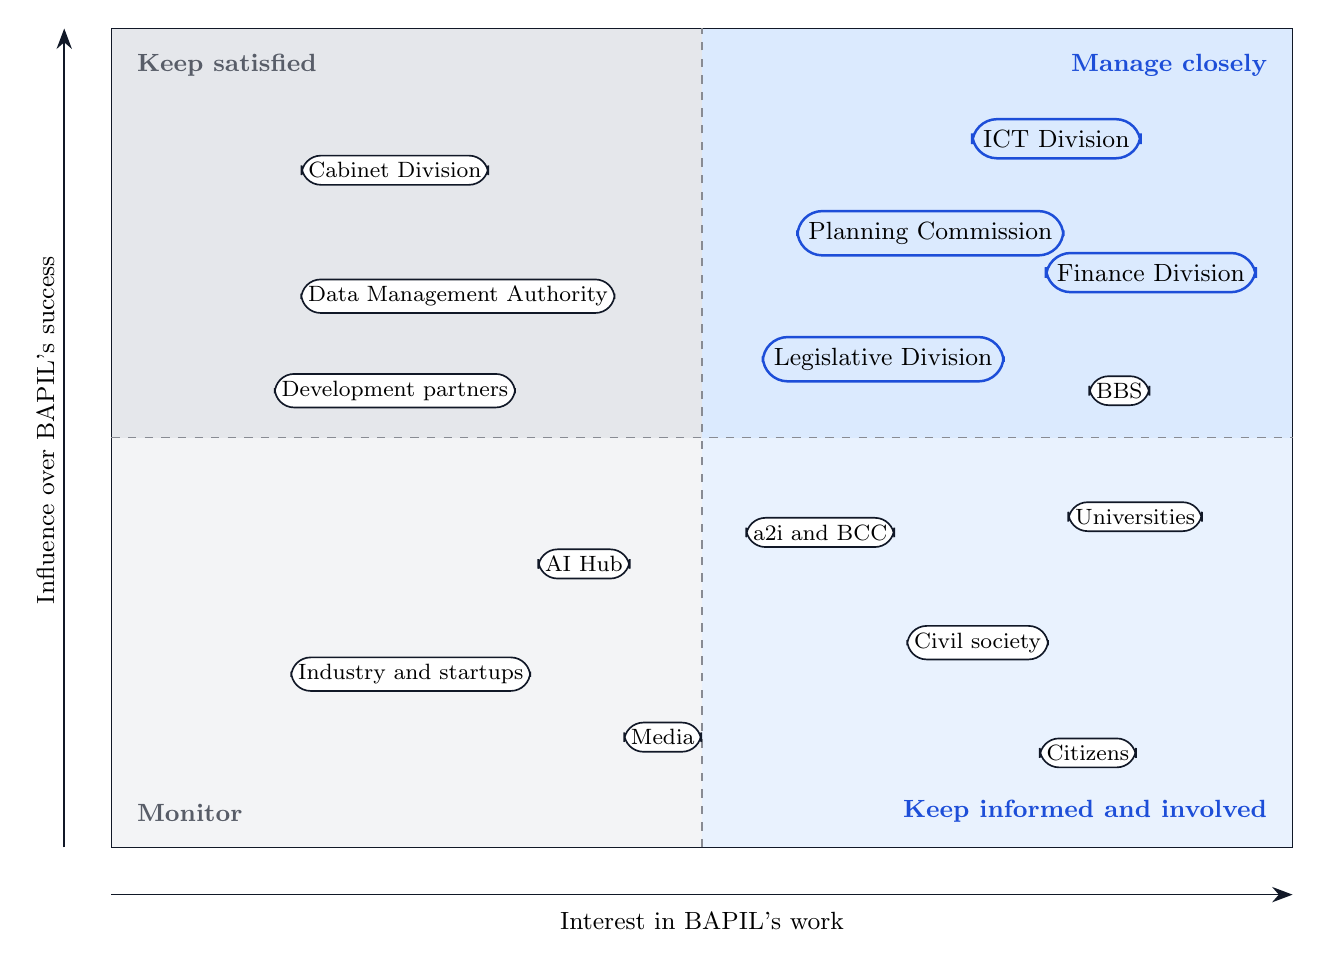
\begin{tikzpicture}
\def\W{150mm}\def\H{104mm}
\fill[band] (0,0) rectangle (0.5*\W,0.5*\H);
\fill[accentlight!60] (0.5*\W,0) rectangle (\W,0.5*\H);
\fill[band2] (0,0.5*\H) rectangle (0.5*\W,\H);
\fill[accentlight] (0.5*\W,0.5*\H) rectangle (\W,\H);
\draw[ink, line width=0.6pt] (0,0) rectangle (\W,\H);
\draw[ink!50, dashed] (0.5*\W,0) -- (0.5*\W,\H);
\draw[ink!50, dashed] (0,0.5*\H) -- (\W,0.5*\H);
\draw[arr] (0,-6mm) -- node[below=1mm, font=\small]{Interest in BAPIL's work} (\W,-6mm);
\draw[arr] (-6mm,0) -- node[above=1mm, font=\small, rotate=90]{Influence over BAPIL's success} (-6mm,\H);
\node[font=\small\bfseries, anchor=north west, text=ink!70] at (2mm,\H-2mm) {Keep satisfied};
\node[font=\small\bfseries, anchor=north east, text=accent] at (\W-2mm,\H-2mm) {Manage closely};
\node[font=\small\bfseries, anchor=south west, text=ink!70] at (2mm,2mm) {Monitor};
\node[font=\small\bfseries, anchor=south east, text=accent] at (\W-2mm,2mm) {Keep informed and involved};
\tikzset{sh/.style={box, rounded corners=7pt, font=\footnotesize, inner sep=2.5pt}, shk/.style={sh, key}}
\node[shk] at (120mm,90mm) {ICT Division};
\node[shk] at (104mm,78mm) {Planning Commission};
\node[shk] at (132mm,73mm) {Finance Division};
\node[sh] at (36mm,86mm) {Cabinet Division};
\node[sh] at (44mm,70mm) {Data Management Authority};
\node[shk] at (98mm,62mm) {Legislative Division};
\node[sh] at (128mm,58mm) {BBS};
\node[sh] at (90mm,40mm) {a2i and BCC};
\node[sh] at (36mm,58mm) {Development partners};
\node[sh] at (130mm,42mm) {Universities};
\node[sh] at (110mm,26mm) {Civil society};
\node[sh] at (60mm,36mm) {AI Hub};
\node[sh] at (38mm,22mm) {Industry and startups};
\node[sh] at (124mm,12mm) {Citizens};
\node[sh] at (70mm,14mm) {Media};
\end{tikzpicture}
\end{document}
